\documentclass[aps,apl,twocolumn,groupedaddress]{revtex4-1}
%\documentclass[12pt]{article}   	% use "amsart" instead of "article" for AMSLaTeX format

\usepackage{graphicx}				% Use pdf, png, jpg, or eps� with pdflatex; use eps in DVI mode
								% TeX will automatically convert eps --> pdf in pdflatex		
%\usepackage{caption}

\begin{document}

\title{Classical Schr\"{o}dinger-like Equation Revisited}
\author{Chris Richardson, Peter Schlagheck, John Martin, Thierry Bastin, Nicolas Vandewalle}
\affiliation{University of Liege}
\date{\today}							% Activate to display a given date or no date

\begin{abstract}

A wave equation which sheds light on the origin of the Schr\"{o}dinger equation has previously been proposed.  This equation which we call the classical Schr\"{o}dinger-like equation is the Schr\"{o}dinger equation plus an extra non-linear term, a classicality-enforcing potential, which has the effect of canceling out all quantum and wave-like effects.  The Schr\"{o}dinger equation has been recovered from the classical Schr\"{o}dinger-like equation by making assumptions which have the effect of completely canceling the classicality-enforcing potential.

We demonstrate both analytically and numerically that it is not strictly necessary to get rid of the classicality-enforcing potential to recover quantum behavior.  We show that by scaling and not necessarily eliminating the classicality-enforcing potential the linear Schr\"{o}dinger equation is recovered, but with a rescaled $\hbar$.  Even though the classical Schr\"{o}dinger-like equation with a scaled classicality-enforcing potential is non-linear, we demonstrate that it behaves in a very linear way.

We call the classical Schr\"{o}dinger-like equation with a scaled classicality-enforcing potential the transition equation and it can be a tool to explore the transition between the quantum and classical worlds.

\end{abstract}

\maketitle

%\section{Explaining the Classical Schr\"{o}dinger-like Equation}
%
%The evolution of a classical particle can be described by its action $S$ which obeys the the Hamilton-Jocobi equation:
%
%\begin{eqnarray}
%\frac{\partial S}{\partial t} &=& \frac{1}{2 m} \nabla S^2 - V \label{eqn:hamilton-jacobi}
%\end{eqnarray}
%
%If we assume instead that the particle has some statistical distribution in space given by $\rho(x,t) = A^2(x,t)$ we can construct a complex valued classical wave function:
%
%\begin{eqnarray}
%\psi_{cl} &=& A e^{\frac{i}{\hbar} S} \label{eqn:classical_wf}
%\end{eqnarray}
%
%This wave function should obbey the continuity equation:
%
%\begin{eqnarray}
%\frac{\partial \rho}{\partial t} &=& - \nabla \cdot j \label{eqn:classical_wf} \nonumber \\
%&=& - \nabla \cdot \frac{\hbar}{i m} \left(\psi^*_{cl} \nabla \psi_{cl}-   \psi_{cl} \nabla \psi^*_{cl} \right)
%\end{eqnarray}
%
%Which gives an equation derived separately by Schleich et al. which they refer to as the Van Vleck continuity equation.  
%
%\begin{eqnarray}
%\frac{\partial A^2(x,t)}{\partial t} + \frac{\partial}{\partial x} \left( \frac{1}{m} \frac{\partial S(x,t)}{\partial x} A^2(x,t) \right)= 0  \label{eqn:Oriols_cons}
%\end{eqnarray}
%
%Combining Eqs.~ (\ref{eqn:hamilton-jacobi}), (\ref{eqn:classical_wf}) and (\ref{eqn:Oriols_cons}) we get the classical Schr\"{o}dinger-like equation:
%
%\begin{eqnarray}
%i \hbar \frac{\partial \psi_{cl}}{\partial t} &=& - \frac{\hbar^2}{2 m} \frac{\partial^2 \psi_{cl}}{\partial x^2} \nonumber \\
%&&+ \left(V + \frac{\hbar^2}{2 m} \frac{1}{\left| \psi_{cl} \right|} \frac{\partial^2 \left| \psi_{cl} \right|}{\partial x^2}\right) \psi_{cl} \label{eqn:class_schrod}
%\end{eqnarray}

\section{Formulation of Theories}

\subsection{Quantum Mechanics}

There are excellent theories to accurately describe the quantum and the classical worlds.  However there are systems such as quandrops which lie squarely in the middle.  Tools to probe this transition area are valuable and we develop such a tool in what follows.

The physical behavior of the very small world is described almost perfectly by quantum mechanics which obeys the Schr\"{o}dinger equation

\begin{eqnarray}
i \hbar \frac{\partial \psi}{\partial t} &=& - \frac{\hbar^2}{2 m} \nabla^2 \psi + V \psi \;, \label{eqn:schrod}
\end{eqnarray}
a linear partial differential equation that describes how a quantum state evolves in time.  $\psi$ is a wavefunction whose modulus squared gives a probability density, $m$ is the mass, $V$ is the potential and $\hbar$ is Plank's constant[cite].  The Schr\"{o}dinger equation leads to behavior that is never observed in classical mechanics such as single particle interference.  This unique behavior can be reformulated as the influence of a potential that describes all quantum behavior which acts on a classical particle.  David Bohm did this in 1999 [cite] by first writing the wavefunction is in it's polar form as

\begin{eqnarray}
\psi &=& A e^{ i S / \hbar }\;, \label{eqn:polarwf}
\end{eqnarray}
where $A$ is a positive real amplitude and $S$ is the action.  Inserting this into the Schr\"{o}dinger equation leads to the modified Hamilton-Jacobi [cite] equation

\begin{eqnarray}
 \frac{\partial S}{\partial t} &=& - \frac{1}{2 m} (\nabla S)^2 - V + \frac{\hbar^2}{2 m} \frac{ \nabla^2 A}{A}\;,
\end{eqnarray}

This differs from the actual Hamilton-Jacobi equation by the term

\begin{eqnarray}
U = - \frac{\hbar^2}{2 m} \frac{ \nabla^2 A}{A} = - \frac{\hbar^2}{2 m} \frac{1}{\left| \psi \right|} \nabla^2 \left| \psi \right| \label{eqn:qm_pot}
\end{eqnarray}
which Bohm termed the \emph{quantum-mechanical potential}~\cite{bib:bohm}.  A classical particle that can be described by Eq.~(\ref{eqn:polarwf}) under the influence of this quantum-mechanical potential will exhibit all the unique behavior we associate with quantum mechanics.

We can take the opposite approach and determine what is necessary to make a quantum sate behave in a purely classical manner.  Interpreting the wave function in Eq.~(\ref{eqn:polarwf}) as a classical probability distribution Oriols and Mompart \cite{bib:obm} derived a wave equation that describes classical physics.  Separately, Schleich et al. \cite{bib:revisited} have also derived the same equation and suggest that the Schr\"{o}dinger equation has its origins in it.  We call it the classical Schr\"{o}dinger-like equation and it is defined as

\begin{eqnarray}
i \hbar \frac{\partial \psi_{cl}}{\partial t} &=& - \frac{\hbar^2}{2 m} \nabla^2 \psi_{cl} \nonumber \\
&+& \left(V + \frac{\hbar^2}{2 m} \frac{1}{\left| \psi_{cl} \right|} \nabla^2 \left| \psi_{cl} \right| \right) \psi_{cl} \;,\label{eqn:class_schrod}
\end{eqnarray}
where the probability density, in analogy to the Schr\"{o}dinger equation, is given from the modulus squared of $\psi_{cl}$.  Eq.~(\ref{eqn:class_schrod}) is equivalent to the Schr\"{o}dinger equation plus an extra non-linear term which has the effect of canceling out all quantum or wave-like effects.  Schleich et al. refer to this term as the \emph{classicality-enforcing potential}.  It is of course Bohm's quantum-mechanical potential, Eq.~(\ref{eqn:qm_pot}), with the opposite sign.  The classical Schr\"{o}dinger-like equation can then be though of as the Schr\"{o}dinger equation with an extra potential that masks all quantum behavior.

There are several ways to explore the transition between these two extremes.  Since $\hbar$ is a purely quantum term that does not show up in classical mechanics it is reasonable to explore what happens when $\hbar \rightarrow 0$.  We can immediately see that the Schr\"{o}dinger equation becomes useless.  The WKB approximation assumes a small $hbar$ by requiring the amplitude $A$ in Eq.~(\ref{eqn:polarwf}) to be slowly varying compared to the phase term $S / \hbar$.  This leads to successful approximate solutions in the semi-classical regime but they become singular near the classical turning point.  We propose to explore the semi-classical transition area by modifying the classical Schr\"{o}dinger-like equation.

Schleich et al. transfer from the non-linear classical Schr\"{o}dinger-like equation, Eq.~(\ref{eqn:class_schrod}),  to the linear Schr\"{o}dinger equation, Eq.~(\ref{eqn:schrod}), by associating the classicality-enforcing potential with the quantum action.  In this way, the classicality-enforcing potential is canceled out in Eq.~(\ref{eqn:class_schrod}).  We would like to add, however, that it is not strictly necessary to get rid of the classicality-enforcing potential to recover quantum behavior.  We have found that by scaling and not necessarily eliminating the classicality-enforcing potential the linear Schr\"{o}dinger equation is recovered, but with a rescaled $\hbar$.

Inserting a degree of quantumness, $0 \leq \epsilon \leq 1$, into Eq.~(\ref{eqn:class_schrod}) allows us to explore the smooth transition from the classical world, $\epsilon = 0$, to the quantum one, $\epsilon = 1$.

\begin{eqnarray}
i \hbar \frac{\partial \psi}{\partial t} &=& - \frac{\hbar^2}{2 m} \nabla^2 \psi \nonumber \\ 
&+& \left(V + (1 - \epsilon) \frac{\hbar^2}{2 m} \frac{1}{\left| \psi \right|} \nabla^2 \left| \psi \right| \right) \psi\label{eqn:class_schrod_ep}
\end{eqnarray}

We call this the transition equation and we will show that for all values of $\epsilon \neq 0$ it exhibits quantum behavior.  To demonstrate this we take two approaches.  First we show analytically that the transition equation is equivalent to the Schr\"{o}dinger equation with a rescaled $\hbar$.  We then explore numerically what the effect of scaling the classicality-enforcing potential has on the interference of two Gaussian wave packets.


%\section{A Classical Schr\"{o}dinger-like Equation}
%
%A differential equation that describes classical (non-quantum, non-wave-like) physics has been derived by Bohm \cite{bib:bohm} and Oriols and Mompart \cite{bib:obm}.  Separately, Schleich et al. \cite{bib:revisited} have also derived the same equation and suggest that the Schr\"{o}dinger equation has its origins in it.  We call it the classical Schr\"{o}dinger-like equation and it is defined as:
%
%\begin{eqnarray}
%i \hbar \frac{\partial \psi_{cl}}{\partial t} &=& - \frac{\hbar^2}{2 m} \nabla^2 \psi_{cl} \nonumber \\
%&&+ \left(V + \frac{\hbar^2}{2 m} \frac{1}{\left| \psi_{cl} \right|} \nabla^2 \left| \psi_{cl} \right| \right) \psi_{cl} \label{eqn:class_schrod}
%\end{eqnarray}
%
%Where the probability in analogy to the Schr\"{o}dinger equation is given from the modulus squared of $\psi$, the classical wave function.  Eq.~(\ref{eqn:class_schrod}) is the Schr\"{o}dinger equation plus an extra non-linear term which has the effect of canceling out all quantum or wave-like effects.  Schleich et al. refer to this term as the \emph{classicality-enforcing potential}.  It is obvious that if this term were absent, Eq.~(\ref{eqn:class_schrod}) reduces to the fully quantum Schr\"{o}dinger equation.
%
%Schleich et al. transfer from this non-linear classical Schr\"{o}dinger-like equation to the linear Schr\"{o}dinger equation by associating the classicality-enforcing potential with the quantum action.  In this way, the classicality-enforcing potential is canceled out in Eq.~(\ref{eqn:class_schrod}).
%
%We would like to add, however, that it is not strictly necessary to get rid of the classicality-enforcing potential to recover quantum behavior.  We have found that by scaling and not necessarily eliminating the classicality-enforcing potential the linear Schr\"{o}dinger equation is recovered, but with a rescaled $\hbar$.
%
%Inserting a degree of quantumness, $0 \leq \epsilon \leq 1$, into Eq.~(\ref{eqn:class_schrod}) allows us to explore the smooth transition from the classical world, $\epsilon = 0$, to the quantum one, $\epsilon = 1$.
%
%\begin{eqnarray}
%i \hbar \frac{\partial \psi}{\partial t} &=& - \frac{\hbar^2}{2 m} \nabla^2 \psi_{cl} \nonumber \\ 
%&&+ \left(V + (1 - \epsilon) \frac{\hbar^2}{2 m} \frac{1}{\left| \psi \right|} \nabla^2 \left| \psi_{cl} \right| \right) \psi \label{eqn:class_schrod_ep}
%\end{eqnarray}
%
%We call this the transition equation and we will show that for all values of $\epsilon \neq 0$ it exhibits quantum behavior.  To demonstrate this we take three approaches.  First we show analytically that the transition equation is equivalent to the Schr\"{o}dinger equation with a rescaled $\hbar$.  We then explore numerically what the effect of scaling the classicality-enforcing potential has on the double slit experiment.  Finally we explore how the transition equation can shed light on the results of a macroscopic quantum experiment.
%
\section{Scaling $\hbar$}

The non-linear transition equation is equivalent to the linear Schr\"{o}dinger equation with a $\hbar$ scaled by the degree of quantumness, $\epsilon$.

\begin{eqnarray}
\tilde{\hbar} = \hbar \sqrt{\epsilon} \label{eqn:hbar_scaled}
\end{eqnarray}

We begin by inserting the polar form of the wave equation, Eq.~(\ref{eqn:polarwf}), into the transition equation, Eq.~(\ref{eqn:class_schrod_ep}), and finding the individual elements.  The Laplacian is:

\begin{eqnarray}
\nabla^2 \psi &=& \big[ \nabla^2 A + 2 \frac{i}{\hbar}  (\nabla A) \cdot (\nabla S) \nonumber \\
&+& \frac{i}{\hbar} A \nabla^2 S - \frac{1}{\hbar^2}  A (\nabla S)^2 \big] e^{ i S / \hbar }
\end{eqnarray}

The time derivative of Eq.~(\ref{eqn:polarwf}) is:

\begin{eqnarray}
i \hbar \frac{\partial \psi}{\partial t} &=& (i \hbar \frac{\partial A}{\partial t} - A \frac{\partial S}{\partial t}) e^{ i S / \hbar }
\end{eqnarray}

And the contribution from the classicality-enforcing potential is:

\begin{eqnarray}
\frac{\psi}{\left| \psi \right|} \nabla^2 \psi &=& (\nabla^2 A) e^{ i S / \hbar }
\end{eqnarray}

Gathering the real and imaginary terms we recover two equations.  The first is the continuity equation:

\begin{eqnarray}
m \frac{\partial A}{\partial t}  &=& - (\nabla A) \cdot (\nabla S) - \frac{1}{2} A \nabla^2 S  \label{eqn:continuity}
\end{eqnarray}

The second is an equation very similar to the Hamilton-Jacobi equation but with the quantum-mechanical potential, Eq.~(\ref{eqn:qm_pot}) , scaled by the degree of quantumness, $\epsilon$:

\begin{eqnarray}
 \frac{\partial S}{\partial t} &=& - \frac{1}{2 m} (\nabla S)^2 - V + \epsilon \frac{\hbar^2}{2 m} \frac{ \nabla^2 A}{A}
\end{eqnarray}

Making the substitution $\tilde{\hbar} = \hbar \sqrt{\epsilon}$ we get:

\begin{eqnarray}
\frac{\partial S}{\partial t} &=& - \frac{1}{2 m} (\nabla S)^2 - V + \frac{\tilde{\hbar}^2}{2 m} \frac{ \nabla^2 A}{A}  \label{eqn:hamilton-jacobi_rescaled}
\end{eqnarray}
which has the effect of canceling out the degree of quantumness.  Eqs.~(\ref{eqn:continuity}) and (\ref{eqn:hamilton-jacobi_rescaled}) are now completely equivalent to the Schr\"{o}dinger equation with a rescaled $\hbar$ and we can write:

\begin{eqnarray}
\psi &=& A e^{i S / \tilde{\hbar}} \\
i \tilde{\hbar} \frac{\partial \psi}{\partial t}  &=& -  \frac{\tilde{\hbar}^2}{2 m} \nabla^2 \psi + V \psi
\end{eqnarray}
 
\section{Exploring the Quantum-Classical Transition for the Interference of Two Wave Packets}

Quantum mechanically, we expect the probability for the particles after the wave packets have spread to be represented by the normal Young interference pattern~\cite{bib:Young} that spreads with time and distance.  For classical particles with no wave nature we expect the particles to behave like baseballs and pass through one or the other slit and continue on without diffraction for all time.  We can explore the transition between these two extremes by solving the transition equation numerically.  For comparison, we first solve the double slit using the fully quantum Schr\"{o}dinger equation.

\subsection{Fully Quantum Wave Packets}

We start the fully quantum analysis with two gaussians, $V = 0$ and initial conditions:

\begin{eqnarray}
i \hbar \frac{\partial \psi}{\partial t} &=& -\frac{\hbar^2}{2 m} \frac{\partial^2 \psi}{\partial x^2}  \\
\psi(x,0) &=& \sqrt{N_0} \left( e^{-\frac{(x-d)^2}{4 \sigma^2}}+e^{-\frac{(x+d)^2}{4 \sigma ^2}}\right) \label{eqn:double_init}
\end{eqnarray}
where $2d$ is the distance between the centers of the Gaussians and $\sigma$ is the width of the Gaussians. The normalization is:

\begin{eqnarray}
 N_0 = 1 / \left(2 \sqrt{2 \pi } \sigma  \left(e^{-\frac{d^2}{2 \sigma ^2}}+1\right)\right)
 \end{eqnarray}

When the time-dependent Schr\"{o}dinger is solved for the initial condition, Eq.~(\ref{eqn:double_init}), the time-dependent wave function is found to be:

\begin{eqnarray}
\psi(x,t) &=& \sqrt{\frac{N_0}{a_t}} \left(e^{-\frac{(x-d)^2}{4 a^2_t}}+e^{-\frac{(x+d)^2}{4 a^2_t}}\right)
\end{eqnarray}
where $a^2_t = 1+i \frac{\hbar}{2 m \sigma^2} t$.  When the modulus is squared the interference term becomes obvious:

\begin{eqnarray}
\left| \psi(x,t) \right|^2 &=& \frac{N_0}{\sigma_t} \Bigg[\left(e^{-\frac{(x-d)^2}{4 \sigma^2_t}}+e^{-\frac{(x+d)^2}{4 \sigma^2_t}}\right)^2 \label{eqn:wf_double_t} \nonumber \\
&-& 4 e^{-\frac{ \left(x^2 + d^2\right)}{2 \sigma^2_t}} \sin^2 \left(\frac{\hbar}{4 m \sigma^2 \sigma^2_t} t x d \right)\Bigg]\end{eqnarray}
were $\sigma^2_t = \frac{\hbar^2}{4 m^2 \sigma^2} t^2 +\sigma^2$ is the time dependent width.  This gives the expected Young interference pattern as can be seen in Fig.~(\ref{fig:diffract_movie}-f).

\subsection{The Semi-Quantum Semi-Classical Wave Packets}

To explore the transitional behavior of the interference of two Gaussian wave packets from the quantum to the classical regime we use the transition equation, Eq.~(\ref{eqn:class_schrod_ep}), with no potential, $V = 0$:

\begin{eqnarray}
i \hbar \frac{\partial \psi}{\partial t} &=& -\frac{\hbar^2}{2 m} \frac{\partial^2 \psi}{\partial x^2} + (1 - \epsilon) \frac{\hbar^2}{2 m} \frac{\psi}{\left| \psi \right|} \frac{\partial^2 \left| \psi \right|}{\partial x^2}  \label{eqn:schrod_class_nov}
\end{eqnarray}

This equation can be solved numerically using the explicit finite difference method.  To do so Eq.~(\ref{eqn:double_init}) is discretized into $\psi_{x_n,0}$ where $x_n = n \Delta x$.  The next time step, $t_n = n \Delta t$, for Eq.~(\ref{eqn:schrod_class_nov}) is given by the recurrence relation:

\begin{eqnarray}
\psi(x_n,t_{n+1}) &=& i \frac{\Delta t}{(\Delta x)^2} \Big[ \psi_{x_{n+1},t_n} + \psi_{x_{n-1},t_n} \nonumber \\
&-& \psi_{x_n,t_n} \left(2 + i \frac{(\Delta x)^2}{\Delta t}\right) \nonumber \\
&-& (1 - \epsilon) \frac{\psi_{x_n,t_n}}{\left|\psi_{x_n,t_n}\right|} \Big(\left| \psi_{x_{n+1},t_n} \right| \nonumber \\
&-&  2 \left| \psi_{x_n,t_n} \right| + \left| \psi_{x_{n-1},t_n} \right| \Big)\Big]
\end{eqnarray}

\begin{figure}[ht]
\begin{minipage}[t]{0.23\textwidth}
%\centering
  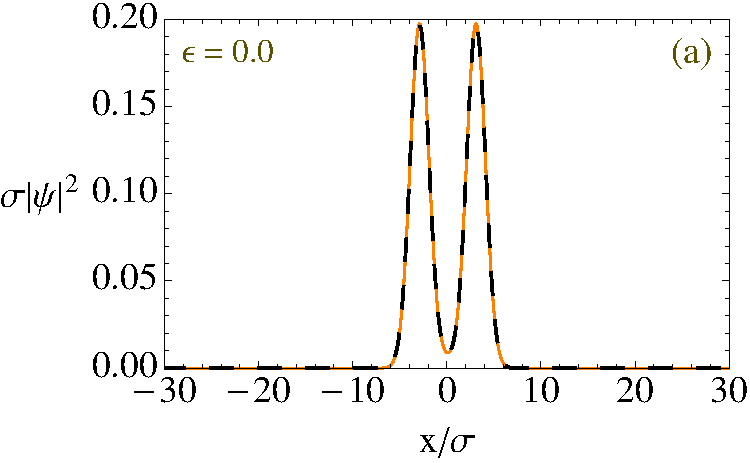
\includegraphics[width=1\textwidth]{Graphics/Probs_ep-10.pdf}
  %\caption*{(a)}
\end{minipage}
\begin{minipage}[t]{0.23\textwidth}
%\centering
  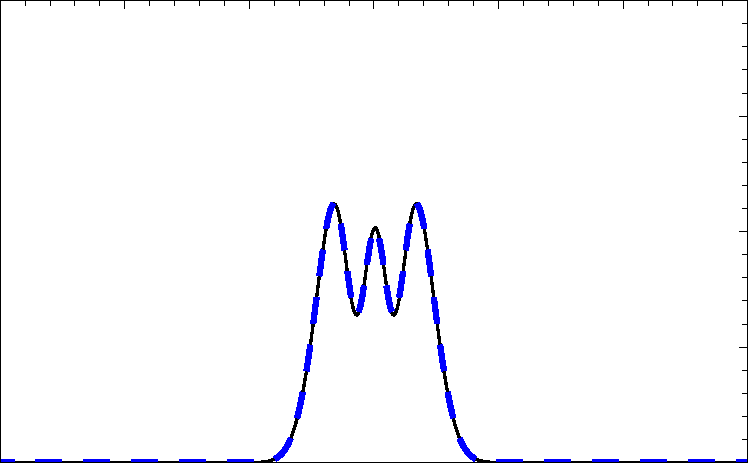
\includegraphics[width=1\textwidth]{Graphics/Probs_ep-98.pdf}
  %\caption*{(b)}
\end{minipage}
\begin{minipage}[t]{0.23\textwidth}
%\centering
  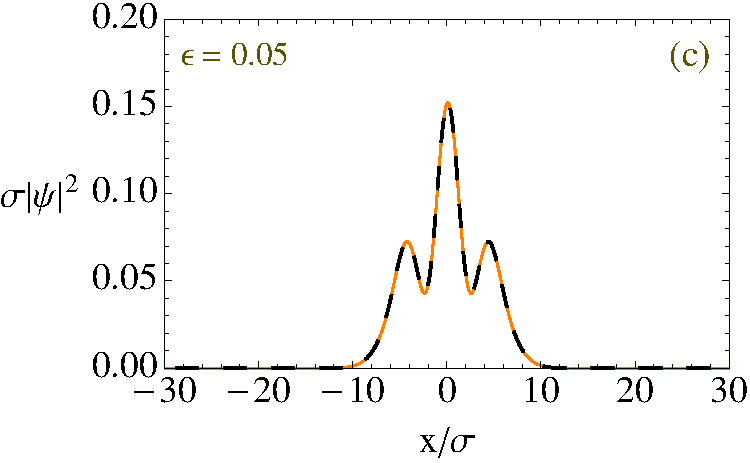
\includegraphics[width=1\textwidth]{Graphics/Probs_ep-95.pdf}
  %\caption*{(c)}
\end{minipage}
\begin{minipage}[t]{0.23\textwidth}
%\centering
  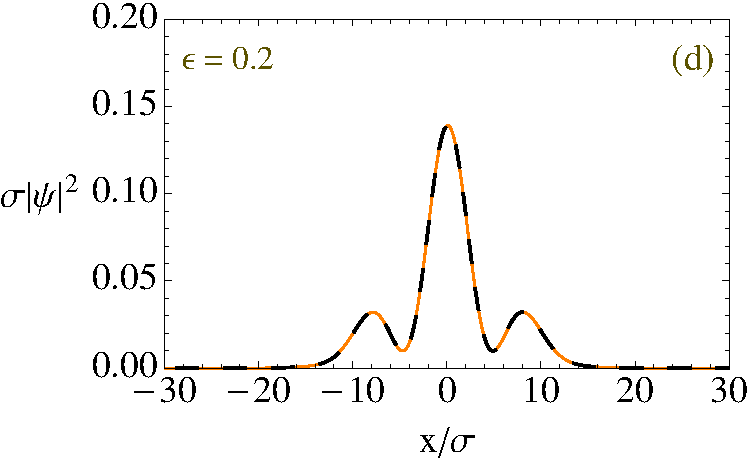
\includegraphics[width=1\textwidth]{Graphics/Probs_ep-8.pdf}
  %\caption*{(d)}
\end{minipage}
\begin{minipage}[t]{0.23\textwidth}
%\centering
  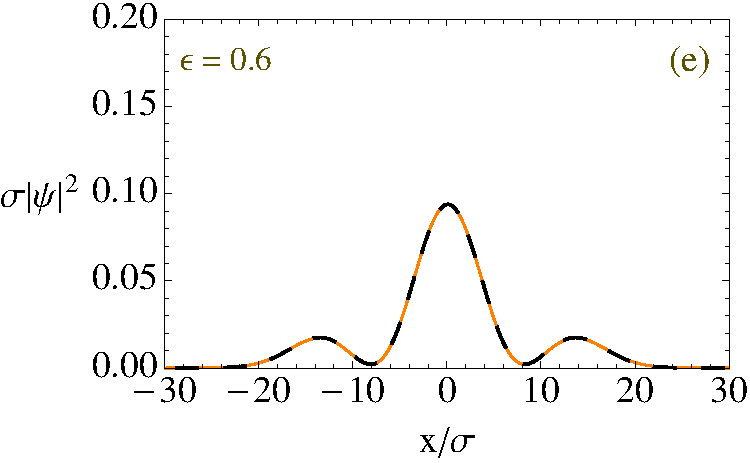
\includegraphics[width=1\textwidth]{Graphics/Probs_ep-4.pdf}
  %\caption*{(e)}
\end{minipage}
\begin{minipage}[t]{0.23\textwidth}
%\centering
  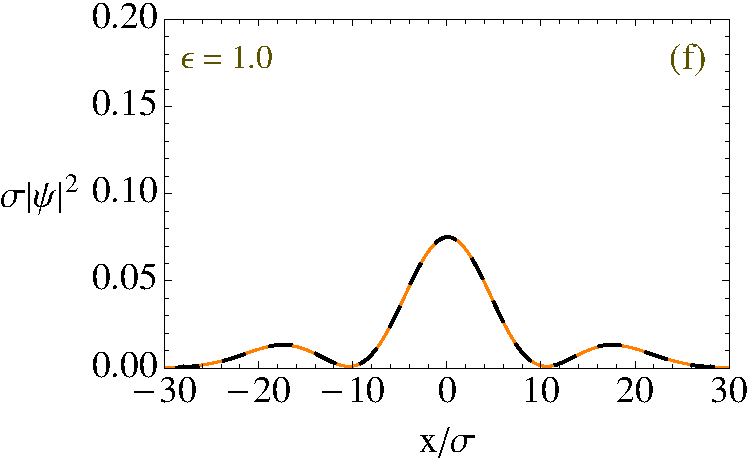
\includegraphics[width=1\textwidth]{Graphics/Probs_ep-0.pdf}
  %\caption*{(f)}
\end{minipage}
\caption{Solid line is the analytic probability density using the Schr\"{o}dinger equation with a scaled $\hbar = \tilde{\hbar} \sqrt{\epsilon}$ and the dashed line is the simulated probability density using the transition equation.  All plots are evaluated at the same time $t = 20 \frac{m \sigma^2}{\hbar}$ and the distance between the center of the two gaussians is $d = 6 \sigma$. Plot (a) is the fully classical case with $\epsilon = 0$. (b) $\epsilon = 0.02$. (c) $\epsilon = 0.05$. (d) $\epsilon = 0.2$. (e) $\epsilon = 0.6$. (f) is for the case $\epsilon = 1$ when $\tilde{\hbar} = \hbar$.}
\label{fig:diffract_movie}
\end{figure}

The asymptotic behavior is as expected.  For the completely quantum case, $\epsilon = 1$, the diffraction pattern that forms, Fig.~(\ref{fig:diffract_movie}-f), is identical to the analytic case, Eq.~(\ref{eqn:wf_double_t}).  For the completely classical case, $\epsilon = 0$, The diffraction pattern that forms, Fig.~(\ref{fig:diffract_movie}-a), is just that of the initial distribution, Eq.~(\ref{eqn:double_init}).

[EXPAND THIS] Fig.~(\ref{fig:diffract_movie}) shows that the linear Schr\"{o}dinger equation with a scaled $\hbar$ produces completely equivalent results to the numerically solved non-linear transition equation.

For all values of $0 < \epsilon \leq 1$, given enough time, a far-field diffraction pattern will develop with a visibility of one.  The time for a diffraction pattern to develop increases to infinity as degree of quantumness diminishes, $\epsilon \rightarrow 0$.  The diffraction patterns for the higher values of $\epsilon$ are less developed that for the lower values, but the visibility for all of them is one.

\section{Conclusion}

We have demonstrate both analytically and numerically that it is not necessary to get rid of the classicality-enforcing potential to recover quantum behavior.  We have found that by scaling and not necessarily eliminating the classicality-enforcing potential the linear Schr\"{o}dinger equation is recovered, but with a rescaled $\hbar$.

[This is a weaker requirement for quantum behavior in classical systems. No longer do the experiments have to reproduce quantum behavior with $\hbar$.  Any value of $\tilde{\hbar} = \hbar \sqrt{\epsilon}$ will do.]

We can instead scale the degree of quantumness, $\epsilon$ in the transition equation to explore the transition to the classical world.  This does leave us with a non-linear equation to solve, but it avoids the problems that arise when using the Schr\"{o}dinger equation with a small $\hbar$.


\begin{thebibliography}{4}

\bibitem{bib:bohm}
D. Bohm, \emph{A Suggested Interpretation of the Quantum Theory in Terms of ``Hidden'' Variables}. I, Phys. Rev. 85, 166 (1952).

\bibitem{bib:obm}
X.Oriols and J.Mompart \emph{Overview of Bohmian Mechanics}pages: 15-147; Chapter 1 of the book \emph{Applied Bohmian Mechanics: From Nanoscale Systems to Cosmology} Editorial Pan Stanford Publishing Pte. Ltd (2012).

\bibitem{bib:revisited}
Wolfgang P. Schleich, Daniel M. Greenberger, Donald H. Kobe, and Marlan O. Scully
\emph{Schr\"{o}dinger equation revisited}
PNAS 2013 110 (14) 5374-5379; published ahead of print March 18, 2013, doi:10.1073/pnas.1302475110

\bibitem{bib:Young}
Thomas Young, emph{Experimental Demonstration of the General Law of the Interference of Light, Philosophical Transactions of the Royal Society of London}, vol 94 (1804).

\bibitem{bib:couder_orbits}
E. Fort, A. Eddi, A. Boudaoud, J. Moukhtar, and Y. Couder, \emph{Path-memory induced quantization of classical orbits}, PNAS 107, 17515 (2010).

%\bibitem{bib:theonlymystery}
%Feynman, Richard P. \emph{Six Easy Pieces} Reading, MA: Addison-Wesley, 1995.

\end{thebibliography}


\end{document}  